\label{sec:4-task3}
\begin{wraptable}{r}{9cm}
%\begin{table}[h!] %[tbhp]
\def\rownumber{} % hack for re-starting row-counter (and skip the header) 
	%\centering
    \caption{TFD calculation of PPINs on full graph or LCC }
    \label{table:tfd}
    \begin{tabular}{ @{ \makebox[2em][r]{\rownumber\space} } | lcc}
    	
		\textbf{Organism} & \textbf{TFD-full} &  \textbf{TFD-LCC} 
        \gdef\rownumber{\stepcounter{magicrownumbers} \arabic{magicrownumbers} } \\
		\midrule
        %$ Anopheles \ gambiae \ PEST $ & 1.0 & 1.0 \\ 
        $ Anopheles \ gambiae \ PEST $ & 1.0 & 1.0 \\ 
        %$ Apis \ mellifera $ & 1.0 & 1.0 \\ 
        $ Arabidopsis \ thaliana \ Columbia $ & 1.936 & 3.68 \\ 
        %$ Bacillus \ subtilis \ 168 $ & 0.585 & 1.0 \\ 
        %$ Bos \ taurus $ & 0.61 & 1.465 \\ 
        %$ Caenorhabditis \ elegans $ & 1.634 & 3.285 \\ 
        %$ Candida \ albicans \ SC5314 $ & 1.176 & 2.649 \\ 
        %$ Canis \ familiaris $ & 0.591 & 1.104 \\ 
        %$ Cavia \ porcellus $ & 0.75 & 0.585 \\ 
        %$ Chlamydomonas \ reinhardtii $ & 1.302 & 2.032 \\ 
        %$ Chlorocebus \ sabaeus $ & 0.892 & 0.955 \\ 
        %$ Cricetulus \ griseus $ & 1.082 & 2.084 \\ 
        %$ Danio \ rerio $ & 0.918 & 2.354 \\ 
        $ Dictyostelium \ discoideum \ AX4 $ & 1.171 & 1.342 \\ 
        %$ Drosophila \ melanogaster $ & 2.66 & 3.838 \\ 
        %$ Emericella \ nidulans \ FGSC \ A4 $ & 1.696 & 2.875 \\ 
        %$ Equus \ caballus $ & 1.0 & 1.0 \\ 
        %$ Escherichia \ coli \ K12 $ & 1.0 & 1.0 \\ 
        %$ Escherichia \ coli \ K12 \ MC4100 \ BW2952 $ & 0.796 & 1.001 \\ 
        %$ Escherichia \ coli \ K12 \ MG1655 $ & 1.303 & 3.31 \\ 
        $ Escherichia \ coli \ K12 \ W3110 $ & 4.913 & 4.913 \\ 
        %$ Gallus \ gallus $ & 1.058 & 2.511 \\ 
        %$ Glycine \ max $ & 1.438 & 2.155 \\ 
        $ Hepatitus \ C \ Virus $ & 3.399 & 3.948 \\ 
        $ Homo \ sapiens $ & 3.469 & 4.725 \\ 
        $ Human \ Herpesvirus \ 1 $ & 2.466 & 2.466 \\ 
        %$ Human \ Herpesvirus \ 2 $ & 0.775 & 0.955 \\ 
        %$ Human \ Herpesvirus \ 3 $ & 1.0 & 1.0 \\ 
        %$ Human \ Herpesvirus \ 4 $ & 1.828 & 2.732 \\ 
        %$ Human \ Herpesvirus \ 5 $ & 1.445 & 2.334 \\ 
        %$ Human \ Herpesvirus \ 6A $ & 0.892 & 1.171 \\ 
        $ Human \ Herpesvirus \ 6B $ & 0.775 & 0.585 \\ 
        %$ Human \ Herpesvirus \ 7 $ & 1.0 & 1.0 \\ 
        %$ Human \ Herpesvirus \ 8 $ & 1.107 & 2.356 \\ 
        $ Human \ Immunodeficiency \ Virus \ 1 $ & 4.395 & 4.395 \\ 
        %$ Human \ Immunodeficiency \ Virus \ 2 $ & 0.908 & 1.281 \\ 
        %$ Human \ papillomavirus \ 16 $ & 1.289 & 1.605 \\ 
        %$ Macaca \ mulatta $ & 1.342 & 1.962 \\ 
        %$ Meleagris \ gallopavo $ & 1.0 & 1.0 \\ 
        %$ Mus \ musculus $ & 2.008 & 3.803 \\ 
        %$ Mycobacterium \ tuberculosis \ H37Rv $ & 1.416 & 1.803 \\ 
        %$ Neurospora \ crassa \ OR74A $ & 1.484 & 1.71 \\ 
        %$ Nicotiana \ tomentosiformis $ & 1.0 & 1.0 \\ 
        %$ Oryctolagus \ cuniculus $ & 1.011 & 2.265 \\ 
        %$ Oryza \ sativa \ Japonica $ & 1.088 & 2.102 \\ 
        %$ Ovis \ aries $ & 1.0 & 1.0 \\ 
        %$ Pan \ troglodytes $ & 1.0 & 1.0 \\ 
        %$ Pediculus \ humanus $ & 1.0 & 1.0 \\ 
        %$ Plasmodium \ falciparum \ 3D7 $ & 1.833 & 2.939 \\ 
        %$ Rattus \ norvegicus $ & 1.383 & 2.956 \\ 
        % $ Ricinus \ communis $ & 0.955 & 0.955 \\ 
         $ Saccharomyces \ cerevisiae \ S288c $ & 4.822 & 4.822 \\ 
        % $ Schizosaccharomyces \ pombe \ 972h $ & 2.558 & 3.882 \\ 
        % $ Selaginella \ moellendorffii $ & 1.518 & 1.518 \\ 
        % $ Simian \ Immunodeficiency \ Virus $ & 1.196 & 1.171 \\ 
        % $ Simian \ Virus \ 40 $ & 1.484 & 1.484 \\ 
        % $ Solanum \ lycopersicum $ & 1.222 & 1.617 \\ 
        % $ Solanum \ tuberosum $ & 0.737 & 0.0 \\ 
        % $ Strongylocentrotus \ purpuratus $ & 2.311 & 2.311 \\ 
        % $ Sus \ scrofa $ & 0.86 & 1.854 \\ 
        % $ Tobacco \ Mosaic \ Virus $ & 0.955 & 0.955 \\ 
        % $ Ustilago \ maydis \ 521 $ & 1.171 & 1.171 \\ 
        % $ Vaccinia \ Virus $ & 0.87 & 0.955 \\ 
        % $ Vitis \ vinifera $ & 1.0 & 1.0 \\ 
        % $ Xenopus \ laevis $ & 1.073 & 2.56 \\ 
        % $ Zea \ mays $ & 0.703 & 0.585 \\ 
                %[1ex] 
		\bottomrule
	\end{tabular}	
%\end{table}
\end{wraptable}
We are now ready to comment on the final part of our project, which is the TFD calculation for various PPINs. After implementing the box covering algorithm, we tested it in two versions of PPINs for each of the $66$ organisms, on the complete graph with isolated nodes or disconnected components, as well as on the largest connected component (LCC). The results could be grouped in the following three cases. Firstly, the fully connected networks which showed no difference, those which had disconnected components but TFD was on similar values and, thirdly, some organism which resulted in significantly different TFD between the whole graph and the largest connected component. 

Table~\ref{table:tfd} summarizes the TFD of several PPIN, for both scenarios. $Anopheles gambiae PEST$ is an organism, among other, whose trivial PPIN -- two nodes with one edge -- is depicted in a TFD of $1$. \textit{HIV-1}, as stated earlier, has a fully connected PPIN and this is in accordance with the equality of the two TFDs.  



\begin{figure}[h]
	\begin{minipage}{0.45\textwidth}
    	\centering
		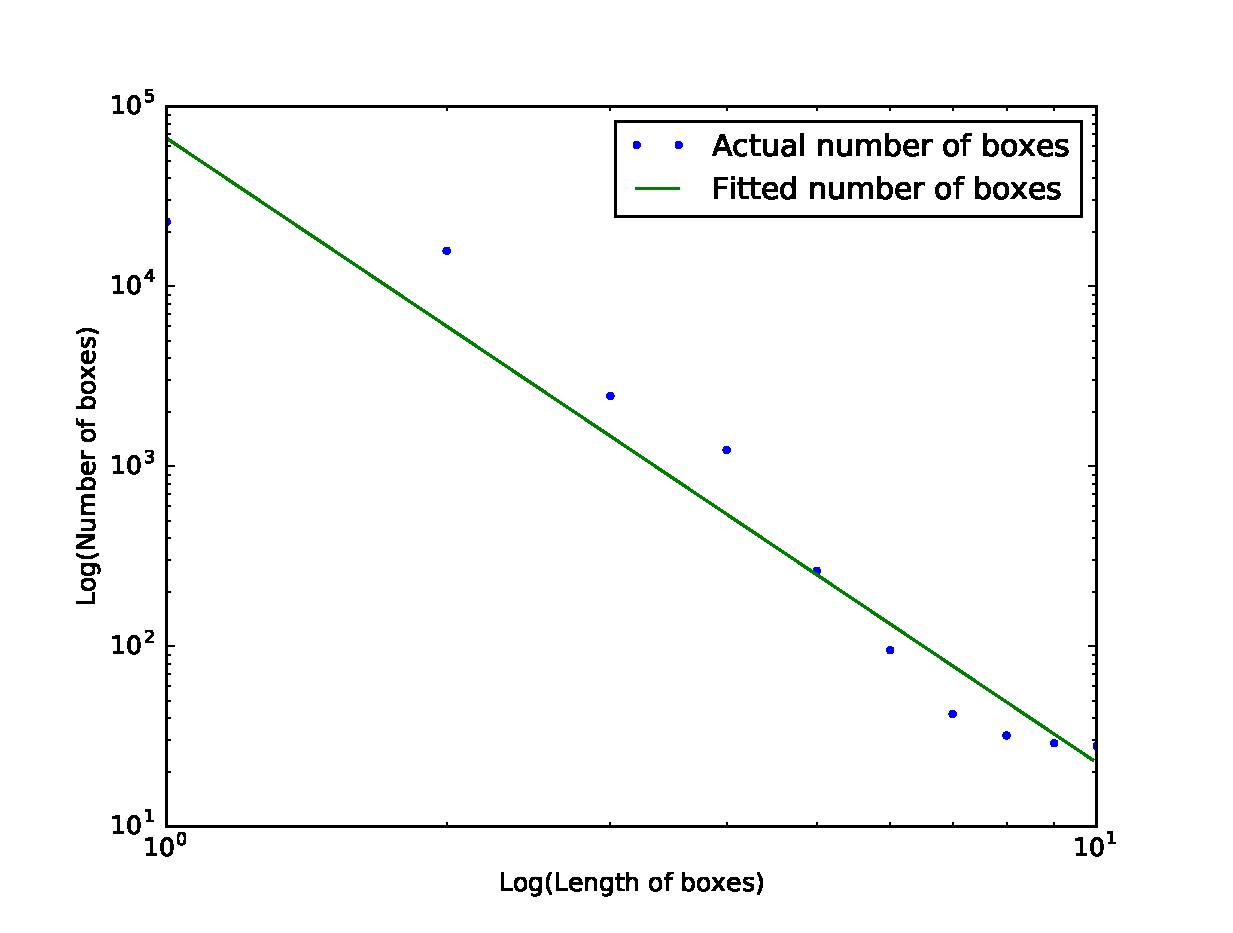
\includegraphics[width=\textwidth]{Graphics/Homo_sapiens_WG.eps}
        \caption{Data fitting on \textit{Homo sapiens} complete PPIN}
        \label{fig:HSWG}
	\end{minipage}
	%\hfill
	\begin{minipage}{0.45\textwidth}
		\centering
		%\vspace{10pt} % Hack for correct positioning
		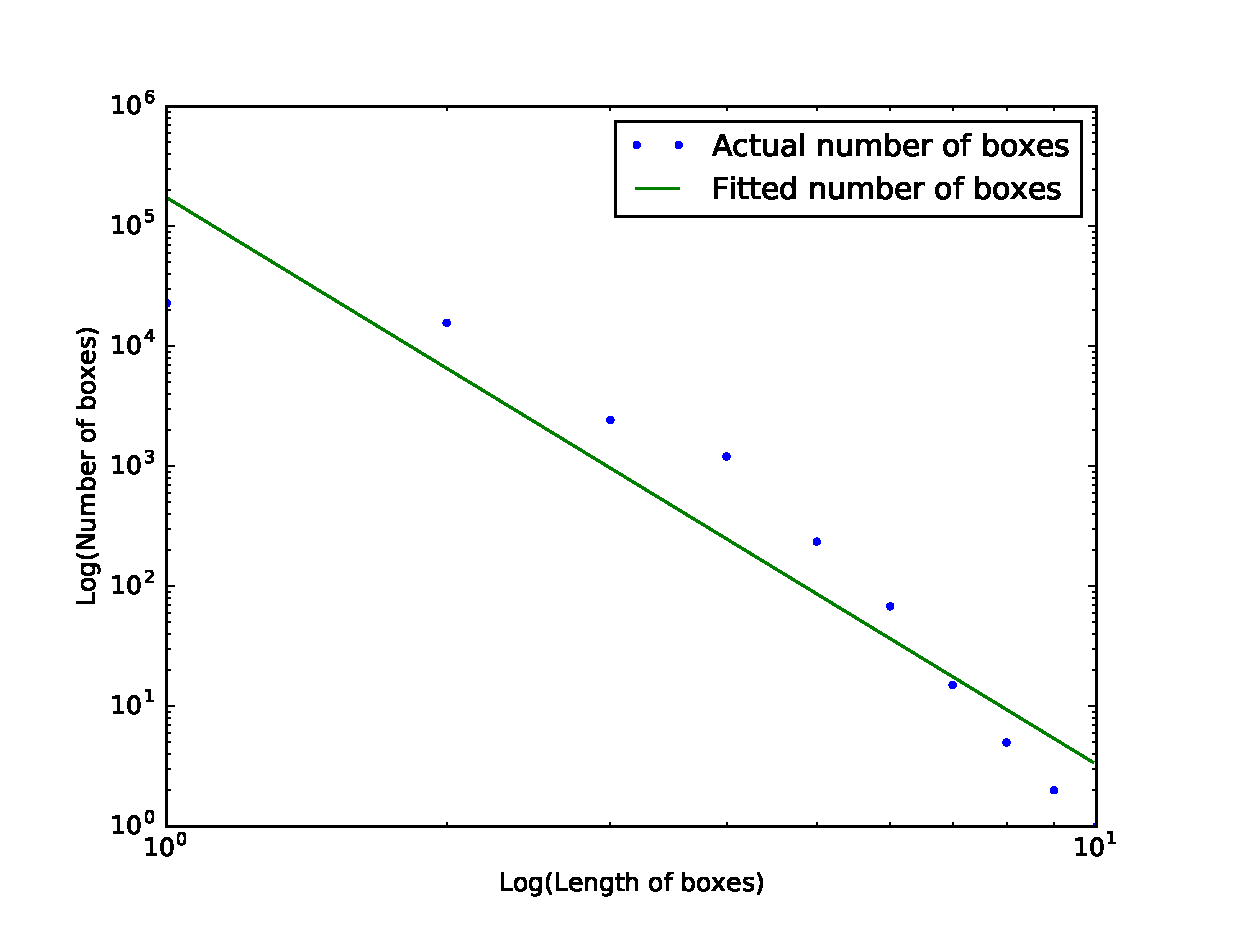
\includegraphics[width=\textwidth]{Graphics/Homo_sapiens_LCC.eps}
        \caption{Data fitting on the largest connected component of Homo sapiens PPIN}
		\label{fig:HSLCC}
	\end{minipage}
\end{figure}

The diagrams of Figures~\ref{fig:HSWG}-\ref{fig:HSLCC} present the number of boxes required for graph covering as a function of the box-side length, in a logarithmic scale. The estimated pairs are depicted as blue dots whereas green lines correspond to the linear-fit approximation.    

\subsection*{Code and Scripts} For the sake of efficiency and productivity we used a \textsc{GitHub} repository \footnote{ \url{github.com/giorkala/Protein-Protein-Interaction-Networks-Project/tree/master/PPIN_Construction}} with all our scripts and functions. After providing the initial dataset, it should work as a pipeline following the directions in comments or descriptions.

%\subsection*{Conclusions}

